\chapter{RESULTS AND DISCUSSION}
\section{RESULTS}
We integrated five sensors and a Bluetooth module micro on a single micro controller and also a Bluetooth module and wifi module on another micro controller.
\subsection{Bluetooth module}
We showed that by using two Bluetooth modules we can communicate between them wirelessly. The data collected from one Bluetooth module is transmitted to another Bluetooth module placed in a certain distance wirelessly.
\subsection{sound sensor:}
We are able to find the variation in the sound in decibel units. We had able to found the sound variation in the machine when it is working efficiently and about to shut down. By using this sound variation of the machine we had programmed a certain value to the sound sensor. When the sound sensor reach the value it alerts the controller that the machine is going to shut down. This also helped in creating a more efficient threshold value.


\newpage
\begin{figure}[h]
\centerline{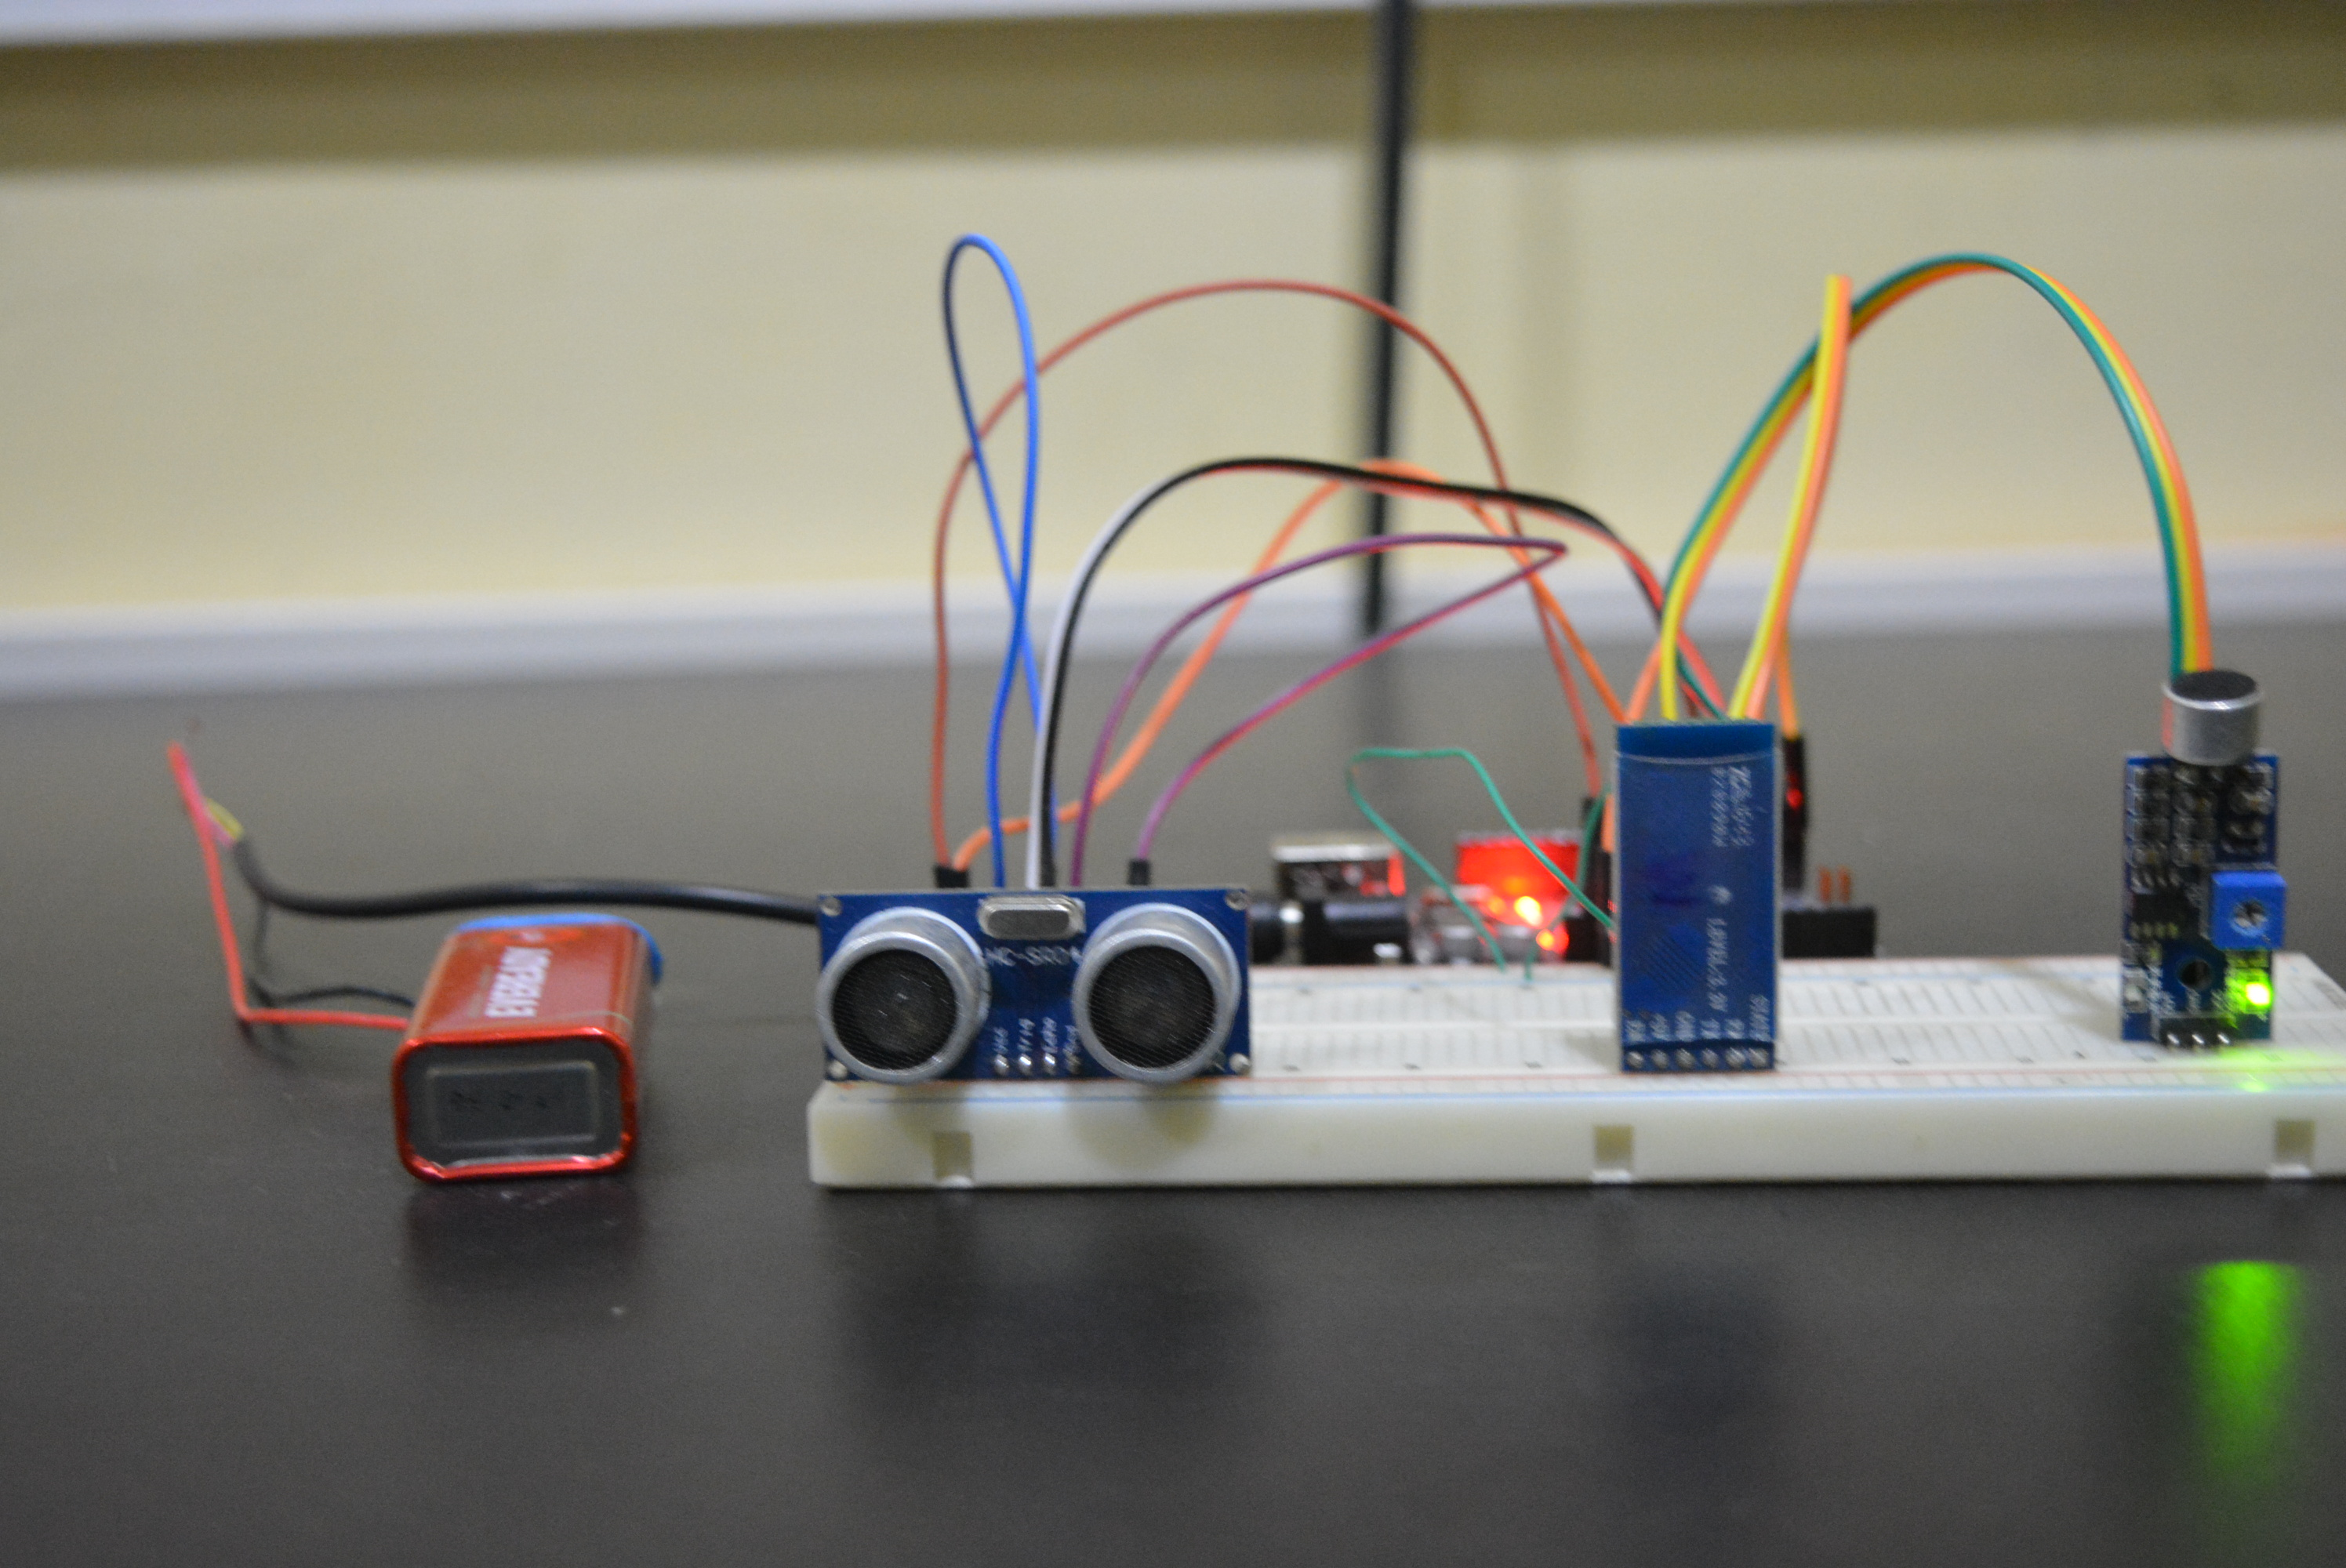
\includegraphics[width=5.7in]{uc}}
\caption{ Sound sensor and ultrasonic sensor embedded in the Arduino board.}
\end{figure}
\subsection{Ultrasonic sensor}
We are able to find distance by using the ultrasonic sensor embedded in the Arduino board. Instead of just calculating just the distance we programmed a certain value to the ultrasonic sensor. The value is determined by the performance of the machine. If the data exceeds the given value it warns the controller. Thus we had prevented the machine to go down to shut down. This helped us to create a threshold value for the machines in the industry.

\begin{figure}[h]
\centerline{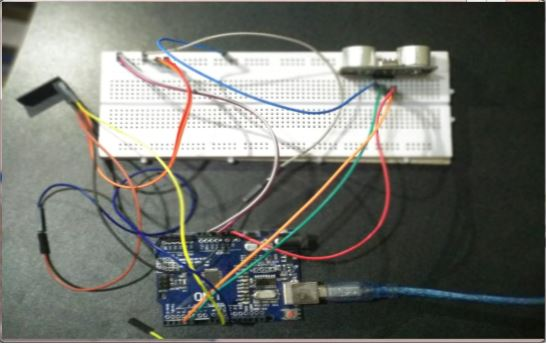
\includegraphics[width=5.7in]{first}}
\caption{Ultrasonic sensor and wi-fi module embedded in the Arduino board.}
\end{figure}
\newpage
\subsection{Cloud}
We are able to collect the data of the machine using sensors. The collected data is stored in the cloud and we had sort the data to create a threshold value for the industrial purposes. To store the data into the cloud we had used Wi-Fi module. 
We had programmed the Wi-Fi module as an access point so we can connect to an internet router. By using the internet we had able to transfer the data from Arduino to cloud.We had sort the data in cloud to set a threshold value by using machine learning. The threshold value is used to increase the efficiency of the machine in industries. The maintenance cost and repair costs of the machines is decreased.

\begin{figure}[h]
\centerline{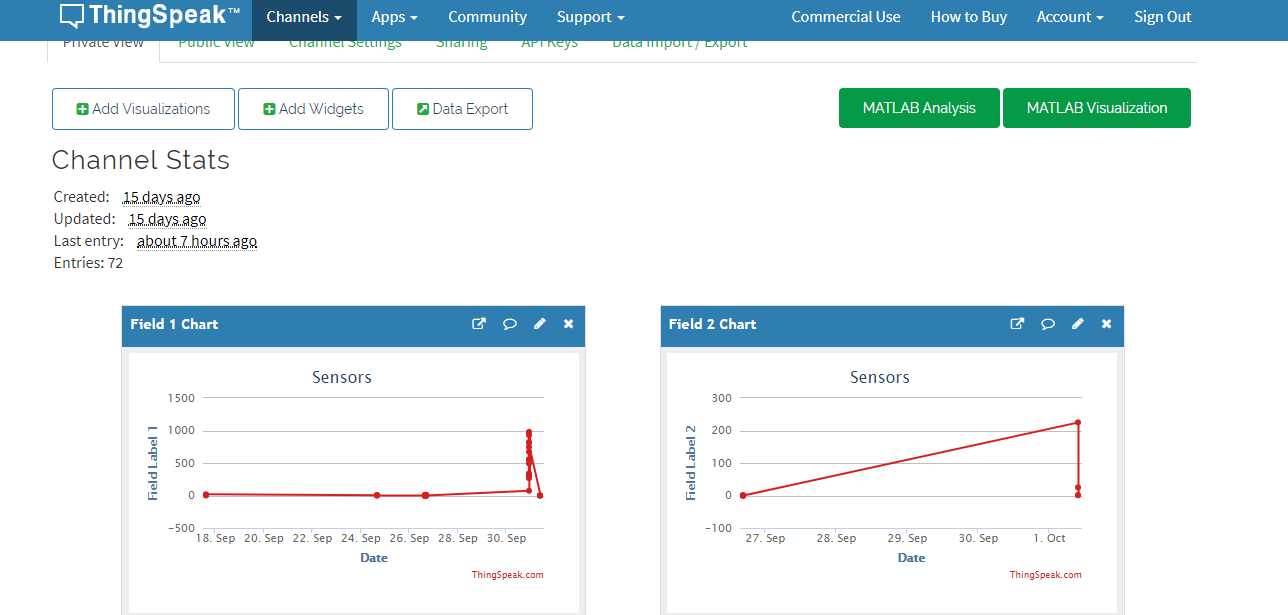
\includegraphics[width=4.7in]{01}}
\caption{Data representation in cloud for two sensors.}
\end{figure}
\begin{figure}[h]
\centerline{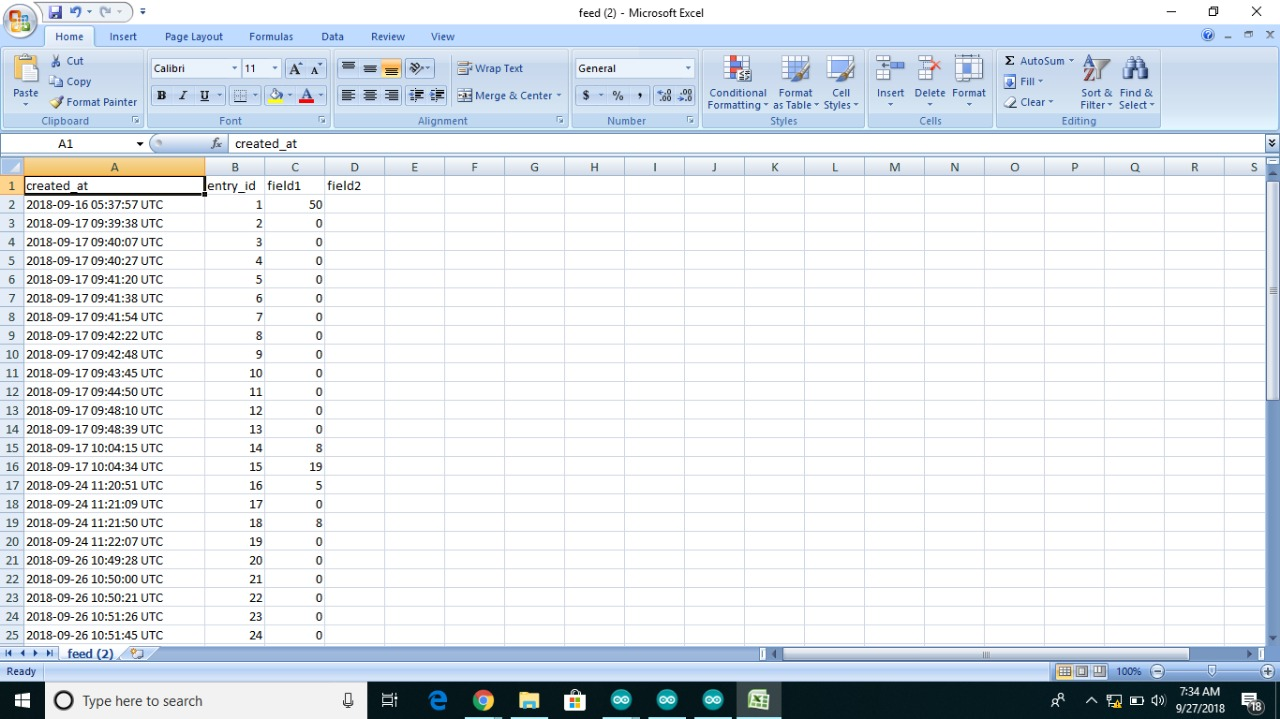
\includegraphics[width=6.7in]{xfortwo}}
\caption{excel sheets from cloud for two sensors}.
\end{figure}
\begin{figure}[h]
\centerline{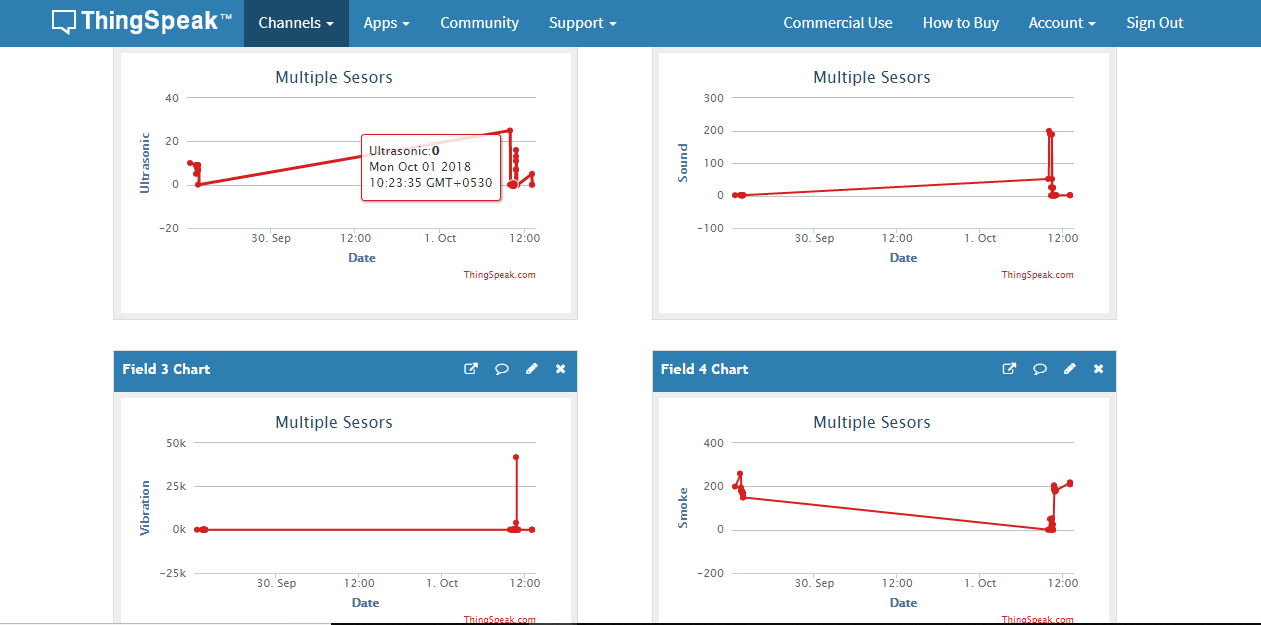
\includegraphics[width=6.7in]{22}}
\caption{Data representation in cloud for multiple sensors.}
\end{figure}
\newpage

\clearpage
\begin{figure}[h]
\centerline{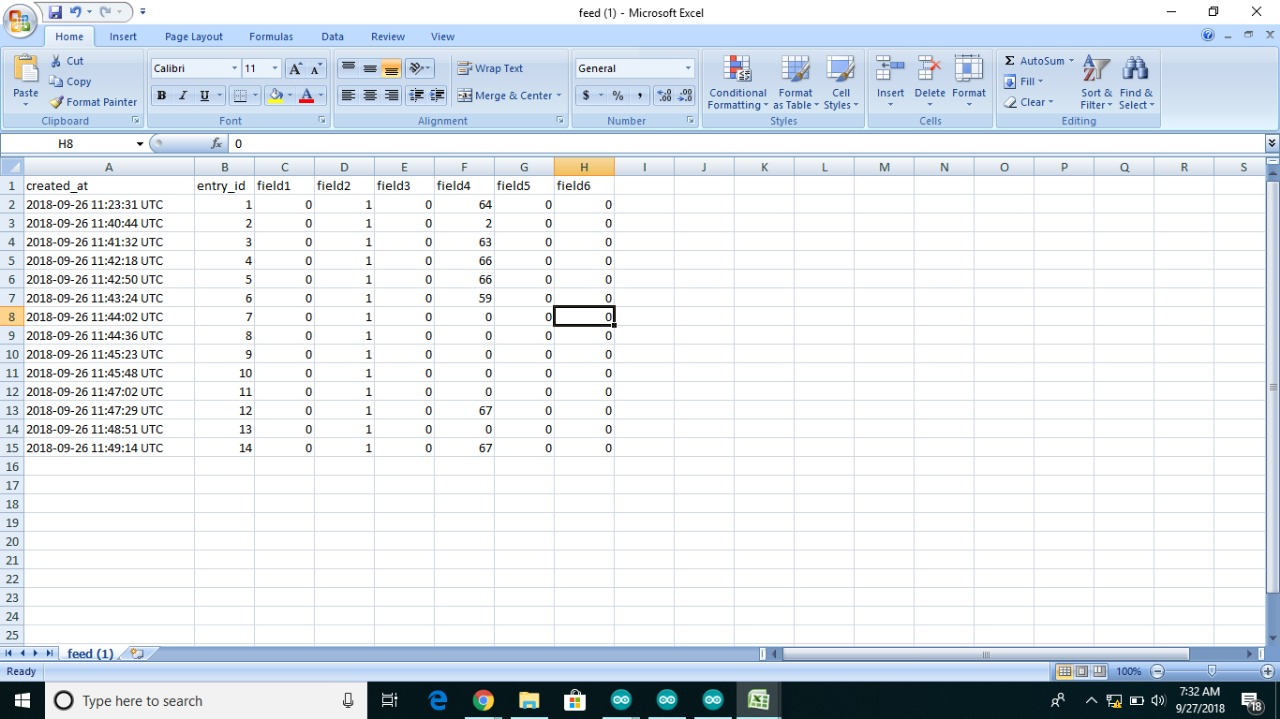
\includegraphics[width=4.7in]{exformultiple}}
\caption{excel sheet from the cloud for multiple sensors.}
\end{figure}


\subsection{WI-FI module }[h]
This wi-fi module we used here mainly to send and receive the data from sensor  to cloud platform .it makes easier for the data transmission which is also a good option with low cost, with some further ideas we will bring more modified and integrated devices which will have more sensors which in turn can be used in all the areas where they can be used for maintenance purpose or for security issues.


Some images of the integrated devices with the sensor embedded on them :

\begin{figure}[h]
\centerline{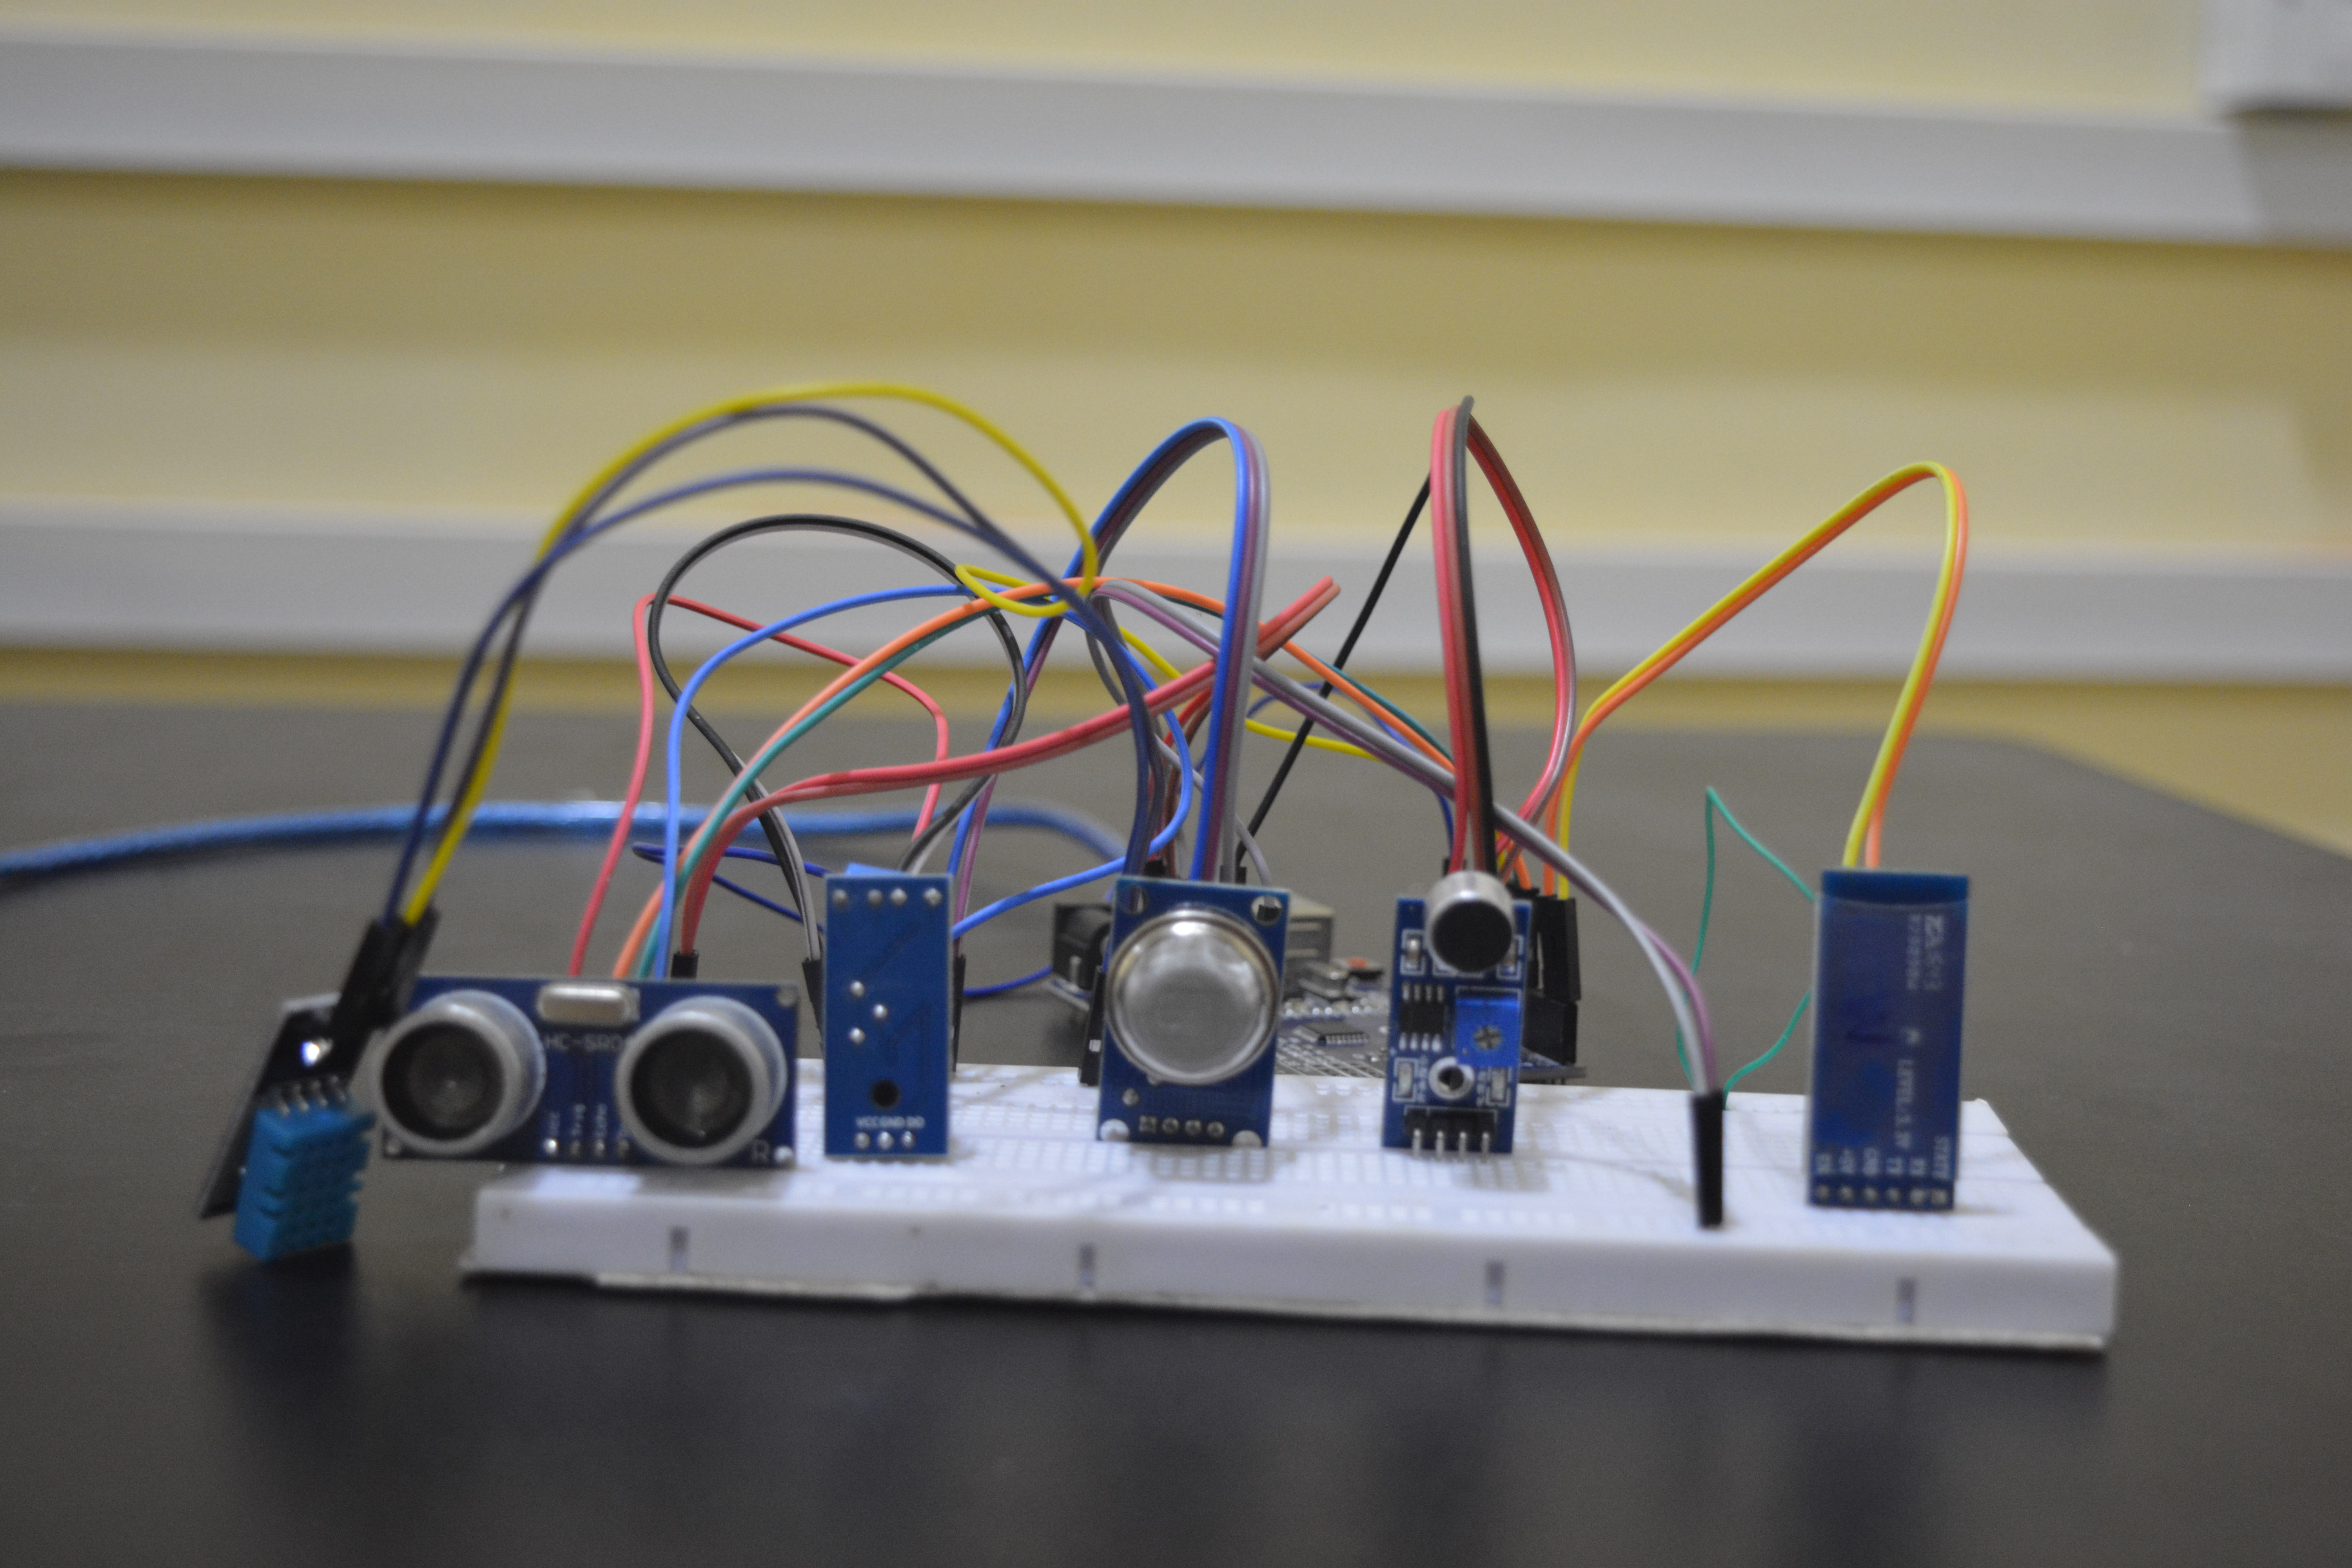
\includegraphics[width=4.7in]{master2}}
\caption{Master device to collect data from the sensors.}
\end{figure}
\vspace{0.3in}
\begin{figure}[h]
\centerline{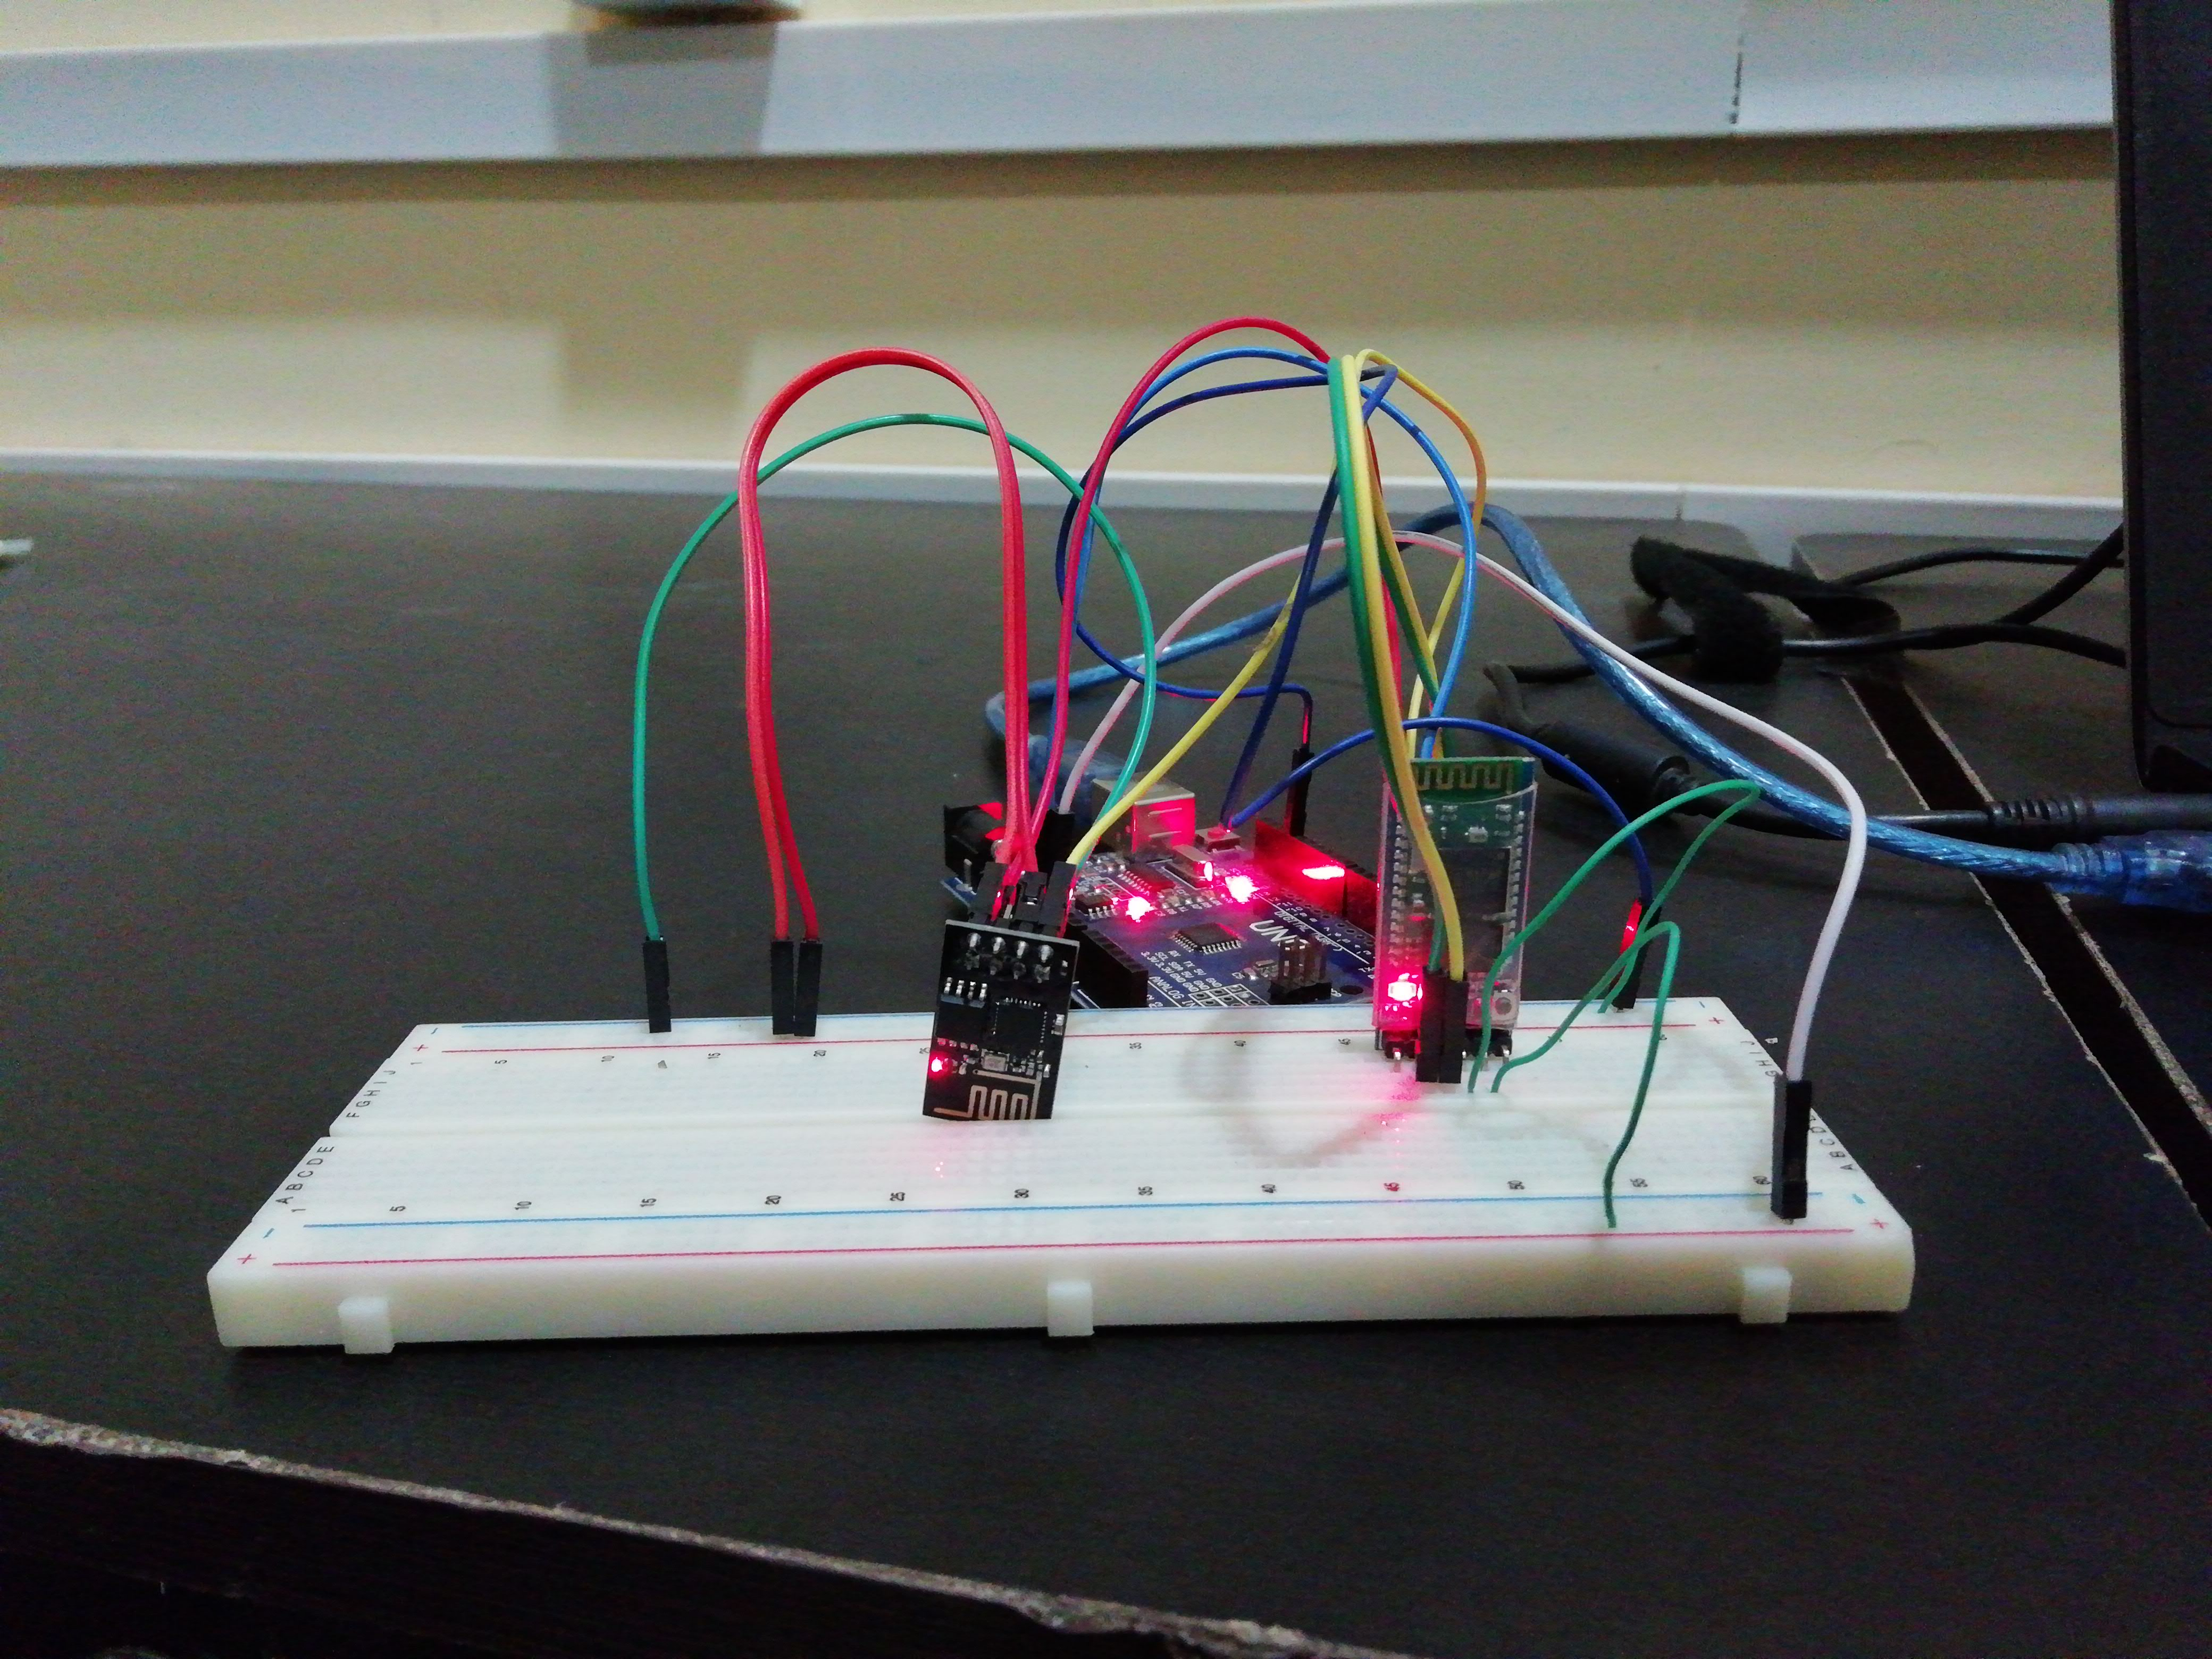
\includegraphics[width=4.7in]{sl}}
\caption{Slave device to transfer data to the cloud.}
\end{figure}
\newpage



\newpage
\section{DISCUSSION}
The external sounds around the machines can change the value of the sound variation in the sound sensors. The threshold value gets affected by it.some other issues that can be considered in all of these are the external parameters which effect for the input we are taking which leads to wrong data leading to wrong predictions .\\
\subsection{FUTURE WORK}
We will add more sensor more sensor to the micro controller and test them in different environments. Our major objective will be to make device more compatible and efficient for larger machines. 